\documentclass{article}
\usepackage{tikz}
\usetikzlibrary{calc}

\begin{document}

Um ponto é \textbf{interior a um triângulo} se é interior a um segmento que tem
por extremidade um vértice e um ponto interior ao lado oposto.

\centering
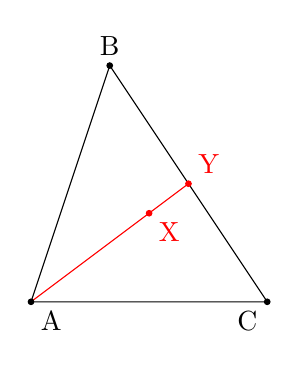
\begin{tikzpicture}
    \coordinate (A) at (0,0);
    \coordinate (B) at (1,3);
    \coordinate (C) at (3,0);

    \coordinate (Y) at ($(B)!0.5!(C)$);
    \coordinate (X) at ($(A)!0.75!(Y)$);

    \draw (A) -- (B) -- (C) -- cycle;

    \draw [red] (A) -- (Y) -- (X);

    \filldraw (A) circle (1pt) node [below right] {A};
    \filldraw (B) circle (1pt) node [above] {B};
    \filldraw (C) circle (1pt) node [below left] {C};

    \filldraw [red] (Y) circle (1pt) node [above right] {Y};
    \filldraw [red] (X) circle (1pt) node [below right] {X};
\end{tikzpicture}

\end{document}
